\chapter{Caching}\label{ch:caching}

\section{Cache Effects}

You need to know about caching
  if your processor is significantly faster than your memory;
  or, more generally, if performing operations is faster than storing data.
And --- guess what ---
  modern processors are awfully fast,
  so you do need to know about caching \citep{blog-cpus-after80s}.
Let's see some strangeness that caching can cause.
Consider the following code:
\begin{ccode}
  for (int i = 0; i < (1 << 27); i += K) arena[i] += 3;
\end{ccode}
Here, \.{arena} is an array of $2^{27}$~integers obtained via \.{mmap}.
The number of operations is proportional to $2^{27}/K$,
  so we expect the runtime to be $\sim 1/K$.
It is:
\begin{center}
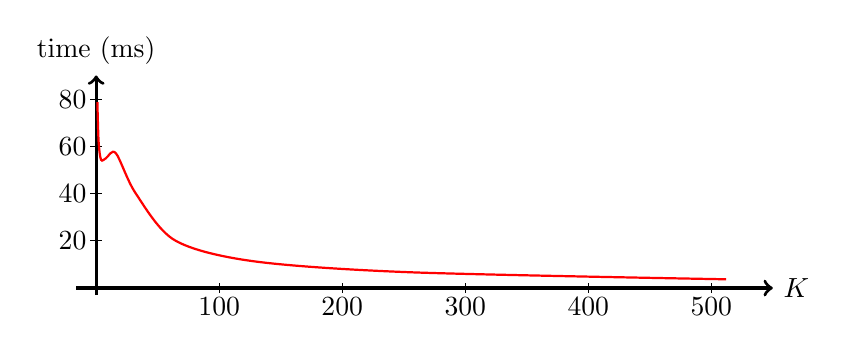
\begin{tikzpicture}[xscale=1/64,yscale=30]
\draw[very thick,->] (0,-0.003) -- (0,0.09) node[above] {time (ms)};
\draw[very thick,->] (-16,0) -- (550,0) node[right] {$K$};
\foreach \y in {20,40,...,80} {
  \draw (-5,\y/1000) -- node[left] {\y} (5,\y/1000);
}
\foreach \x in {100,200,...,500} {
  \draw (\x,-0.002) -- node[below] {\x} (\x,+0.002);
}
\draw[thick,red] plot[smooth]
  coordinates
  { (1,0.078707)
    (2,0.061865)
    (4,0.054286)
    (8,0.054973)
    (16,0.057106)
    (32,0.040196)
    (64,0.020200)
    (128,0.011338)
    (256,0.006670)
    (512,0.003713) };
%    (1024,0.001500) };
\end{tikzpicture}
\end{center}
Except that something funny happens for very small~$K$.
Let's take a closer look there.
\begin{center}
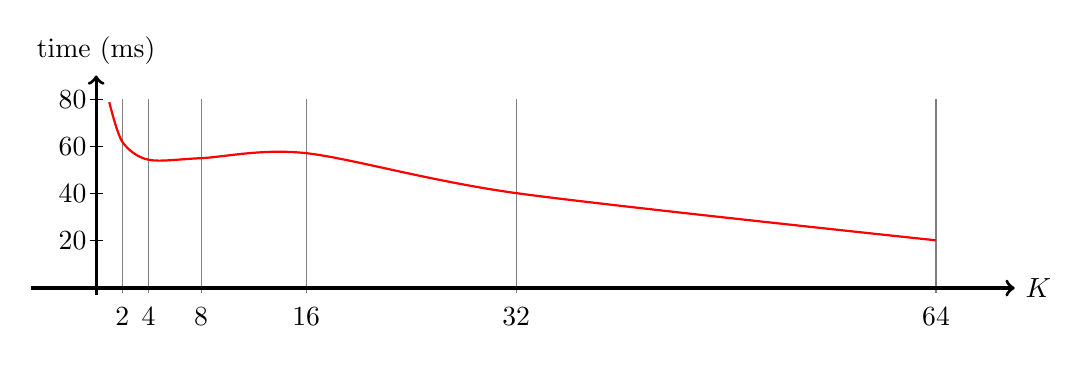
\begin{tikzpicture}[xscale=1/6,yscale=30]
\foreach \y in {20,40,...,80} {
  \draw (-0.5,\y/1000) -- node[left] {\y} (0.5,\y/1000);
}
\foreach \x in {2,4,8,16,32,64} {
  \draw[thin,gray] (\x,-0.002) node[black,below] {\strut\x} -- (\x,+0.08);
}
\draw[very thick,->] (0,-0.003) -- (0,0.09) node[above] {time (ms)};
\draw[very thick,->] (-5,0) -- (70,0) node[right] {$K$};
\draw[thick,red] plot[smooth]
  coordinates
  { (1,0.078707)
    (2,0.061865)
    (4,0.054286)
    (8,0.054973)
    (16,0.057106)
    (32,0.040196)
    (64,0.020200) };
\end{tikzpicture}
\end{center}
The runtime goes down by $20\%$ when $K$ goes up from~$1$~to~$2$,
  but then it appears to stay constant as $K$ further increases.
Only after $K$ passes the threshold of $16$
  does the runtime begin to decrease again.

Here is a plausible explanation.
Recall, from the architecture lectures,
  that memory is organised in a hierarchy:
  at one end we have fast and small memory (registers),
  at the other end we have slow and big memory (hard drives).
The information between two adjacent memory levels is transferred in chunks.
The key to understanding the behaviour observed above,
  is to realise that what matters is
    \emph{how many} chunks are transferred between different levels of the hierarchy.
In other words,
  the runtime of the program from above is dominated by cache faults.
To understand cache faults,
  let us look in more detail at caches.


\section{Ideal Cache Model}

Caches are everywhere.
There is a cache between registers and RAM;
  TLB is a cache used to implement the virtual memory;
  virtual memory itself can be seen as a cache;
  RAM acts as a cache for your hard drive;
  your browser uses a cache;
  a standard technique to solve algorithmic questions is \df{memoization},
    which means using a cache;
  web servers use distributed caches.
Without these caches, your computer and your Internet would be painfully slow.
Thus, caches are important in practice.

We will study caches from a theoretical point of view.
What does this mean?
It means that we focus on some characteristics
  that all of the example caches from above share.
There will also be differences; for example,
  TLB is a cache implemented in hardware,
  while distributed caches are implemented in software
    and involve a fair amount of network use.
These differences, which are what sets apart one cache from another,
  could be the subject of an entire module.

Because caches are so important in practice but also so varied,
  theoreticians became interested in the following question:
How should we design our programs such that they take advantage of available caches
  \emph{without having to tell them which caches are available}?
We do not want to write a program that works well with caches of type
  A, B, C, and D because a cache of type~E might come along soon
  and require a complete rewrite of our program.
We want to write programs that work well with \emph{any} cache.
If you are interested in how to do so,
  the keywords to search for are `cache-oblivious algorithms'.
The definition we will use for an ideal cache
  is from a seminal paper on such algorithms \citep{cache-oblivious}.

\begin{figure} % fig:ideal-cache <<<
\begin{center}
\begin{tikzpicture}\small
  \tikzset{n/.style={thick,rounded corners}}
  \tikzset{g/.style={very thin,gray}}
  \tikzset{m/.style={thick,>=stealth',shorten <=1pt,shorten >=1pt}}
  \draw[n] (0,0) rectangle node[rotate=90] {user} (1,4);
  \draw[n] (5,0) rectangle node[rotate=90] {cache} (6,4);
  \draw[n] (10,0) rectangle node[rotate=90] {backing store} (11,4);

  \foreach \y in { 0.25,0.5,0.75,...,3.75} {
    \draw[g] (5,\y)--(6,\y);
    \draw[g] (10,\y)--(11,\y);
  }
  \draw[g] (5,0) -- (5,-0.5) (6,0) -- (6,-0.5);
  \draw[m,<->] (5,-0.4) -- node[below] {lines, of $L$~words} (6,-0.4);
  \draw[g] (4,4) -- (5,4) (4,0) -- (5,0);
  \draw[m,<->] (4.1,0) --
    node[rotate=90,anchor=south west,pos=0] {$Z/L$ cache lines} (4.1,4);
  \draw[g] (10,0) -- (10,-0.5) (11,0) -- (11,-0.5);
  \draw[m,<->] (10,-0.4) -- node[below] {chunks, of $L$~words} (11,-0.4);
  \draw[g] (11,0) -- (12,0) (11,4) -- (12,4);
  \draw[m,<->] (11.9,0) --
    node[rotate=90,anchor=north west,pos=0] {$X/L$ chunks} (11.9,4);

  \draw[m,<->,>=open triangle 60] (1,3) -- (5,3);
  \draw[m,<->,>=open triangle 60] (6,3) --
    node[below=1ex,text width=3.25cm,align=center]
    {$Q$ cache faults (for an \emph{optimal} replacement strategy)} (10,3);
\end{tikzpicture}
\end{center}
\caption{Ideal Cache Model}
\label{fig:ideal-cache}
\end{figure}
% >>>

The $(Z,L)$ \df{ideal cache} model is illustrated in \autoref{fig:ideal-cache}:
The user thinks it interacts with a backing store
  which is an array of $X$~words.
So, the user issues a sequence of commands:
  read (tell me what word is at index~$i$) and write (put word~$w$ at index~$i$).
A cache handles these commands, pretending it is the backing store.
The cache can often answer faster than the backing store would
  because it has a fast local storage:
  a set of $Z/L$ arrays of size~$L$, which are called \df{cache lines}.
Correspondingly, the backing store is split into chunks of length~$L$:
  chunk~$k$ is a sub-array of the backing store from index $kL$ to index $(k+1)L-1$.
Each cache line is in one of $1+X/L$ possible states:
  either it is empty, or it is mapped to some chunk~$k$.
(The meaning of `line~$\ell$ is mapped to chunk~$k$' will become clear later.
  For now, just think that line~$\ell$ has a tag that says
  either `mapped to~$k$' or `empty'.)
The cache can change the state of a cache line via two operations:
\begin{enumerate}
\item
  If a cache line~$\ell$ is empty,
  then copying the content of chunk~$k$ into line~$\ell$
    makes line~$\ell$ mapped to chunk~$k$.
  We say that chunk~$k$ was \df{loaded} into line~$\ell$.
\item
  If cache line~$\ell$ is mapped to chunk~$k$,
  then copying the content of line~$\ell$ into chunk~$k$ makes the line empty.
  We say that line~$\ell$ was \df{evicted}.
\end{enumerate}
The cache ensures that distinct lines are not mapped to the same chunk.

Although not part of the definition of an ideal cache,
  let us make some remarks about the typical values of $L$, $Z$, and $X$ in practice:
  $L > 1$ and $X \gg Z$.
(1)~Cache lines hold more than word in order to exploit \df{locality of reference},
  which is the tendency of memory accesses that are close in time
  to also be close in space.
(2)~If a cache could hold all the data in the backing store,
  then the cache would not be needed.
Even more, because caches tend to be so expensive compared to the backing store,
  they are significantly smaller.

Suppose now that the user tries to access chunk~$k$.
The cache will:
\begin{enumerate}
\item
  Ensure that there is a line~$\ell$ which is mapped to chunk~$k$.
  It does so as follows:
  \begin{enumerate}
  \item \label{lookup-step}
    if there exists a line~$\ell$ that is mapped to chunk~$k$,
    then there is nothing to do [cache hit]
  \item otherwise [cache miss (or \df{fault})]
    \begin{enumerate}
    \item \label{evict-step}
      if all lines are nonempty, then pick a line~$\ell$ and evict it
    \item
      load chunk~$k$ into some empty line~$\ell$
    \end{enumerate}
  \end{enumerate}
\item Access line~$\ell$, as if it was chunk~$k$.
\end{enumerate}
Which cache line is evicted in Step~\ref{evict-step}?
The ideal cache is clairvoyant:
  it always makes its choices in a way that minimizes the total number of faults.
The intention of this definition is to free us
  from thinking about any particular implementation of the cache,
  when we analyse a program that uses the cache.
This is good because often actual implementations of the cache are complicated
  and because often we don't even know what the implementation is.

\section{Associativity and Replacement}

Any real cache, be it implemented in hardware or software,
  needs to specify algorithms for two operations:
\begin{itemize}
\item \emph{lookup}:
  how to find chunk~$k$ in the cache (Step~\ref{lookup-step})?
\item \emph{eviction}:
  how to choose a cache line to evict (Step~\ref{evict-step})?
\end{itemize}

\smallskip

Lookup could work going through each cache line, looking for a certain chunk~$k$.
That, however, would be inefficient.
In software, it is almost certainly be slow;
  in hardware, this full search could be implemented in parallel,
    which would make it faster,
    but at the cost of having to add a lot of complicated circuitry.
A typical solution is to restrict the set of cache lines where a chunk may reside
  based on its number~$k$.
For example,
  one could decide that chunk~$k$ may only be loaded in line $k \bmod (Z/L)$.
Of course,
  this means that out of two chunks $k_1$~and~$k_2$
    with $k_1 \equiv k_2 \pmod{Z/L}$
  at most one may be in cache at any one time.
Or, one could decide that chunk $k$ may be loaded in line $k\cdot p \bmod (Z/L)$
  and any of the next $9$~positions,
  where $p$~is a fixed prime number.

There are many possible choices, and they fall in three categories.
If a chunk can be in any line, then we say that cache is \df{fully associative}.
If a chunk~$k$ can be only in line~$f(k)$, for some fixed function~$f$,
  then we say that the cache uses \df{direct mapping}.
For anything in-between,
  when a chunk has several lines available but not all,
  we say the cache is \df{set associative}.
The basic tradeoff is this:
  if we restrict more where a chunk may reside,
  then we can implement cache lookup faster
  but at the cost of making it impossible for certain sets of memory locations
    to be stored in the cache.

\smallskip

Now let us move to eviction.
We saw that the ideal cache is clairvoyant.
Of course, no real cache is.
So, do real caches have much more faults than the ideal cache?
No.
It turns out that simple and widely used replacement algorithms
  stay within a constant factor of the theoretical optimum.
To make this statement precise,
  we need to look at a few specific replacement algorithms.
\begin{itemize}
\item {\bf MIN}: evict the line which is last to be referenced again (in the future)
\item {\bf FIFO}: evict the oldest line,
  where age is measured since the line was loaded
  ({\bf f}irst {\bf i}n {\bf f}irst {\bf o}ut)
\item {\bf LRU}: evict the line that was {\bf l}east {\bf r}ecently {\bf u}sed.
\end{itemize}
\begin{figure}
  \tikzset{a/.style={thick,>=stealth}}
  \tikzset{g/.style={thin,dotted}}
  \tikzset{c/.style={fill=red}}
\noindent
\rlap{(i)}\hskip5em
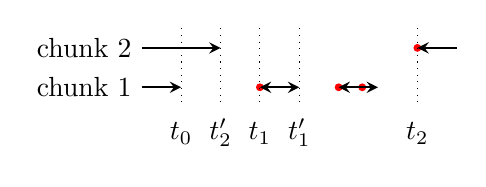
\begin{tikzpicture}[scale=0.5,baseline]
  \path[c]
    (6,1) circle (0.1)
    (2,0) circle (0.1)
    (4,0) circle (0.1)
    (4.6,0) circle (0.1)
  ;

  \draw[a,->] (-1,1) -- node[left,pos=0] {chunk~$2$} (1,1);
  \draw[a,<-] (6,1) -- (7,1);

  \draw[a,->] (-1,0) -- node[left,pos=0] {chunk~$1$} (0,0);
  \draw[a,<->] (2,0) -- (3,0);
  \draw[a,<->] (4,0) -- (5,0);

  \draw[g] (0,1.5) -- (0,-0.5) node[below] {\strut$t_0$};
  \draw[g] (1,1.5) -- (1,-0.5) node[below] {\strut$t'_2$};
  \draw[g] (2,1.5) -- (2,-0.5) node[below] {\strut$t_1$};
  \draw[g] (3,1.5) -- (3,-0.5) node[below] {\strut$t'_1$};
  \draw[g] (6,1.5) -- (6,-0.5) node[below] {\strut$t_2$};
\end{tikzpicture}
\qquad becomes \qquad
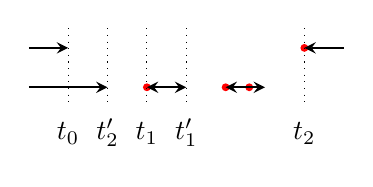
\begin{tikzpicture}[scale=0.5,baseline]
  \path[c]
    (6,1) circle (0.1)
    (2,0) circle (0.1)
    (4,0) circle (0.1)
    (4.6,0) circle (0.1)
  ;

  \draw[a,->] (-1,1) -- (0,1);
  \draw[a,<-] (6,1) -- (7,1);

  \draw[a,->] (-1,0) -- (1,0);
  \draw[a,<->] (2,0) -- (3,0);
  \draw[a,<->] (4,0) -- (5,0);

  \draw[g] (0,1.5) -- (0,-0.5) node[below] {\strut$t_0$};
  \draw[g] (1,1.5) -- (1,-0.5) node[below] {\strut$t'_2$};
  \draw[g] (2,1.5) -- (2,-0.5) node[below] {\strut$t_1$};
  \draw[g] (3,1.5) -- (3,-0.5) node[below] {\strut$t'_1$};
  \draw[g] (6,1.5) -- (6,-0.5) node[below] {\strut$t_2$};
\end{tikzpicture}

\bigskip\noindent
\rlap{(ii)}\hskip5em
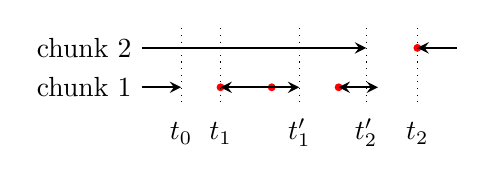
\begin{tikzpicture}[scale=0.5,baseline]
  \path[c]
    (6,1) circle (0.1)
    (1,0) circle (0.1)
    (2.3,0) circle (0.1)
    (4,0) circle (0.1)
  ;

  \draw[a,->] (-1,1) -- node[left,pos=0] {chunk~$2$} (4.7,1);
  \draw[a,<-] (6,1) -- (7,1);

  \draw[a,->] (-1,0) -- node[left,pos=0] {chunk~$1$} (0,0);
  \draw[a,<->] (1,0) -- (3,0);
  \draw[a,<->] (4,0) -- (5,0);

  \draw[g] (0,1.5) -- (0,-0.5) node[below] {\strut$t_0$};
  \draw[g] (1,1.5) -- (1,-0.5) node[below] {\strut$t_1$};
  \draw[g] (3,1.5) -- (3,-0.5) node[below] {\strut$t'_1$};
  \draw[g] (4.7,1.5) -- (4.7,-0.5) node[below] {\strut$t'_2$};
  \draw[g] (6,1.5) -- (6,-0.5) node[below] {\strut$t_2$};
\end{tikzpicture}
\qquad becomes \qquad
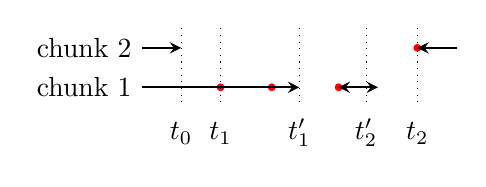
\begin{tikzpicture}[scale=0.5,baseline]
  \path[c]
    (6,1) circle (0.1)
    (1,0) circle (0.1)
    (2.3,0) circle (0.1)
    (4,0) circle (0.1)
  ;

  \draw[a,->] (-1,1) -- node[left,pos=0] {chunk~$2$} (0,1);
  \draw[a,<-] (6,1) -- (7,1);

  \draw[a,->] (-1,0) -- node[left,pos=0] {chunk~$1$} (3,0);
%  \draw[a,<->] (1,0) -- (3,0);
  \draw[a,<->] (4,0) -- (5,0);

  \draw[g] (0,1.5) -- (0,-0.5) node[below] {\strut$t_0$};
  \draw[g] (1,1.5) -- (1,-0.5) node[below] {\strut$t_1$};
  \draw[g] (3,1.5) -- (3,-0.5) node[below] {\strut$t'_1$};
  \draw[g] (4.7,1.5) -- (4.7,-0.5) node[below] {\strut$t'_2$};
  \draw[g] (6,1.5) -- (6,-0.5) node[below] {\strut$t_2$};
\end{tikzpicture}

\bigskip\noindent
\rlap{(iii)}\hskip5em
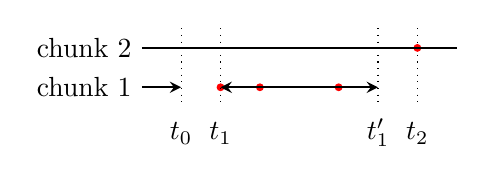
\begin{tikzpicture}[scale=0.5,baseline]
  \path[c]
    (6,1) circle (0.1)
    (1,0) circle (0.1)
    (2,0) circle (0.1)
    (4,0) circle (0.1)
  ;

  \draw[a] (-1,1) -- node[left,pos=0] {chunk~$2$} (7,1);

  \draw[a,->] (-1,0) -- node[left,pos=0] {chunk~$1$} (0,0);
  \draw[a,<->] (1,0) -- (5,0);

  \draw[g] (0,1.5) -- (0,-0.5) node[below] {\strut$t_0$};
  \draw[g] (1,1.5) -- (1,-0.5) node[below] {\strut$t_1$};
  \draw[g] (5,1.5) -- (5,-0.5) node[below] {\strut$t'_1$};
  \draw[g] (6,1.5) -- (6,-0.5) node[below] {\strut$t_2$};
\end{tikzpicture}
\qquad becomes \qquad
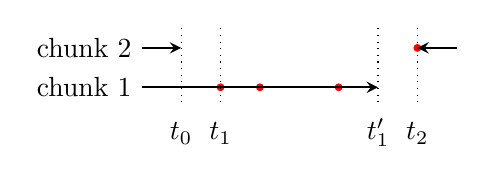
\begin{tikzpicture}[scale=0.5,baseline]
  \path[c]
    (6,1) circle (0.1)
    (1,0) circle (0.1)
    (2,0) circle (0.1)
    (4,0) circle (0.1)
  ;

  \draw[a,->] (-1,1) -- node[left,pos=0] {chunk~$2$} (0,1);
  \draw[a,<-] (6,1) -- (7,1);

  \draw[a,->] (-1,0) -- node[left,pos=0] {chunk~$1$} (5,0);

  \draw[g] (0,1.5) -- (0,-0.5) node[below] {\strut$t_0$};
  \draw[g] (1,1.5) -- (1,-0.5) node[below] {\strut$t_1$};
  \draw[g] (5,1.5) -- (5,-0.5) node[below] {\strut$t'_1$};
  \draw[g] (6,1.5) -- (6,-0.5) node[below] {\strut$t_2$};
\end{tikzpicture}
\caption[Illustrations for the proof of \autoref{th:min-is-best}.]{
  Illustrations for the proof of \autoref{th:min-is-best}.
  An arrow
    \tikz[baseline]{\draw[>=stealth,thick,<->] (0em,0.5ex)--(2em,0.5ex);}
    represents the time there exists a cache line mapped to a certain chunk.
  Faults occur when a chunk is loaded in memory,
    so they are represented by the left ends of the arrows
    \tikz[baseline]{\draw[>=stealth,thick,<-] (0em,0.5ex)--(1em,0.5ex);}.
  A red circle
    \tikz[baseline]{\path[fill=red] (0,0.5ex) circle (2pt);}
    represents an access to a chunk.
}
\label{fig:min-is-best}
\end{figure}

MIN replacement is just as good as the ideal cache.
\begin{theorem}[{\citep{art-belady1966}}]\label{th:min-is-best}
The replacement algorithm MIN achieves a minimum number of cache faults.
\end{theorem}
\begin{proof}[Proof$\,{}^\ast$]
Consider a run of the cache that does not correspond to MIN replacement.
If we follow the eviction decisions taken in the given run,
  then we find a first point in time where the run evicts a different line
    than MIN replacement would.
Let $n$ be the number of cache faults in the given run.
We will show how to produce another run that agrees with MIN replacement
  on a strictly longer prefix.
Moreover, the number of cache faults in the modified run will be $\le n$.
If we apply our transformation repeatedly,
  then eventually we obtain a run that agrees with MIN replacement.
Moreover, the number of cache faults in this run will also be $\le n$.
We can start this process with any run,
  including with one that has a minimum number of faults.
It follows that at least some run that agrees with MIN replacement is optimal.
It's easy to see that all runs that agree with MIN replacement have the same
  number of cache faults,
  and hence all runs that agree with MIN replacement are optimal.

It remains to describe the transformation mentioned above.
Let $t_0$ be the smallest time where the given run disagrees with MIN replacement.
Without loss of generality,
  let $t_0=0$ and let the chunk being accessed be chunk~$0$;
  moreover, suppose the run evicts (a line mapped to) chunk~$1$,
  and MIN replacement is consistent with evicting chunk~$2$.
Let $t_1$ be the time when chunk~$1$ is accessed again,
  and let $t_2$ be the time when chunk~$2$ is accessed again.
Let $t'_1$ be the time when the chunk loaded at time~$t_1$ is evicted.
Let $t'_2$ be the time when chunk~$2$ is first evicted.
So,
\begin{align*}
  t_1 & = \min\{\,t\mid\text{$t>0$ and chunk~$1$ is accessed at time~$t$}\,\} \\
  t_2 & = \min\{\,t\mid\text{$t>0$ and chunk~$2$ is accessed at time~$t$}\,\} \\
  t'_1 &= \min\{\,t\mid\text{$t>{\color{red} t_1}$ and chunk~$1$ is evicted at time~$t$}\,\} \\
  t'_2 &= \min\{\,t\mid\text{$t>{\color{red} 0}$ and chunk~$2$ is evicted at time~$t$}\,\}
\end{align*}
We take $\min\emptyset=\infty$.
Because MIN replacement is consistent with evicting chunk~$2$ at~$t_0$,
  but not consistent with evicting chunk~$1$ at~$t_0$,
  we know that $t_1<t_2$.

Instead of evicting chunk~$1$ at~$t_0$, we evict chunk~$2$ at~$t_0$.
We need to say when chunk~$1$,
  which is now in memory immediately after~$t_0$,
is evicted:
  if $t'_2<t_1$, then we evict it at~$t'_2$;
  if $t'_2\ge t_1$, then we evict it at~$t'_1$.
We need to say when chunk~$2$,
  which is now not in memory immediately after~$t_0$,
is loaded:
  at~$t_2$.

We do not overflow the cache:
  chunk~$1$ is in a line for some extra time,
  but only before $\min\{t_1,t'_2\}$ when chunk~$2$ occupied a line in the given run.
We do not have more faults:
  The only fault that could be introduced by our transformation is at~$t_2$,
  and that happens in the case $t_2<t'_2$ in which case a fault disappears at~$t_1$.
Finally, the transformed run evicts a line only if the original run evicted a line
  at that time.
\todo{simplify proof}
\end{proof}
\autoref{fig:min-is-best} shows several instances of the transformation described
  in the proof from above.

MIN replacement may be just as good as the ideal cache,
  but it is also just as un-implementable.
The following result tells us that two implementable replacement algorithms,
  FIFO and LRU, are not much worse than MIN\null.
\begin{theorem}[{\citep{art-sleator1985}}]\label{th:fifo-lru-almost-optimal}
Consider a fixed but arbitrary sequence of memory accesses.
Let $f$~be the number of cache faults for the MIN replacement algorithm
  with a $(Z,L)$~cache.
Then the number of cache faults for the FIFO (or LRU) replacement algorithm with a $(2Z,L)$~cache
  is~$\le2f$.
\end{theorem}
\todo{Add proof.}
%The proof~[5] is not as easy as that of \autoref{th:min-is-best}.

Informally, \autoref{th:fifo-lru-almost-optimal}
  says that the FIFO and the LRU replacement algorithms are almost optimal.
So, let us look at some examples of how FIFO and LRU work.

\subsection*{FIFO and LRU}

This is an example of how a FIFO cache functions:
\begin{align*}
\def\f#1{{\color{red}#1}}
\def\t#1{\overset{#1}{\to}}
[] \t{\f2} [2] \t{\f0} [20] \t{\f1} [201] \t{2} [201] \t{\f3} [013] \t{1} [013]
  \t{0} [013] \t{0} [013] \t{3} [013] \t{3} [013]
\end{align*}
It looks complicated, but all you need to do is understand the notation.
A bracketed expression like $[201]$ means that
  the cache contains three nonempty lines that are mapped, respectively,
  to chunks $2$, $0$, and~$1$.
We also assume that each nonempty cache line has a timestamp,
  and that cache lines are listed in increasing order of their timestamps.
For example, the cache line that is mapped to chunk~$2$ has the oldest timestamp.
A transition like $\overset{\vbox to 0pt{\vss\hbox{$\scriptstyle2$}\vskip-2pt}}{\to}$ represents an access to chunk~$2$.
Finally, the chunk is \textcolor{red}{red},
  as in $\overset{\vbox to 0pt{\vss\hbox{$\scriptstyle\color{red}2$}\vskip-2pt}}{\to}$,
  when the access caused a cache fault.

We call the string of chunks that are accessed the \df{reference string}.
In the example above, the reference string is $2012310033$.
Let us see how does LRU handle the same reference string,
  using again a cache with three lines:
\begin{align*}
\def\f#1{{\color{red}#1}}
\def\t#1{\overset{#1}{\to}}
[] \t{\f2} [2] \t{\f0} [20] \t{\f1} [201] \t{2} [012] \t{\f3} [123] \t{1} [231]
  \t{\f0} [310] \t{0} [310] \t{3} [103] \t{3} [103]
\end{align*}
Note that the chunk last accessed appears at the right side of the cache:
  look for the pattern $\overset{x}{\to}[\dots x]$.

For both FIFO and LRU,
  the line that is evicted comes from the left side of the cache,
  in our notation.
Exploiting such regularities,
  it is possible to give a common description to FIFO and LRU\null.
Both FIFO and LRU associate a timestamp with each cache line.
When a line needs to be evicted,
  both FIFO and LRU choose the cache line with the oldest (smallest) timestamp.
FIFO and LRU differ only in how they set the timestamps.
FIFO sets the timestamp of a cache line when that line is loaded;
LRU sets the timestamp of a cache line every time that line is accessed.

The previous description of FIFO and LRU
  emphasizes the similarity of the two replacement algorithms.
However, this similarity is at a conceptual level ---
  we do not want to actually implement FIFO and LRU using timestamps,
  because it would be too slow.


\section{LRU and Cache Size}

Once we fix our gaze on two particular replacement algorithms,
  LRU and FIFO,
  several natural questions arise.
Is LRU always better than FIFO?
Is FIFO always better than LRU?
What about on average?
Is FIFO/LRU ever hurt by increasing the cache size?
Most of these are left as exercises below.
(Try them!)
Here, we discuss only one ---
  whether LRU is ever hurt by increasing the cache size.
The answer is no.

\begin{theorem}\label{thm:lru-monotone}
Consider a fixed but arbitrary sequence of memory accesses.
Fix the replacement algorithm to be LRU\null.
Let $f_1$ be the number of faults for a $(Z,L)$~cache,
  and let $f_2$ be the number of faults for a $(Z+L,L)$~cache.
Then, $f_1 \ge f_2$.
\end{theorem}

The idea of the proof is to note that the content of a LRU cache
  coincides, as a set, with some suffix of the reference string.
Without loss of generality, we take $L=1$.
Let $x_1,x_2,x_3,\ldots$ be the reference string,
  and let $C^Z_k$ be the content of an LRU cache of size~$Z$
    after processing the first $k$~elements of the reference string.
We have, for example,
\begin{align}
  C^0_k &= \emptyset
    &&\text{for all $k$}
\\
  C^1_k &= \{x_k\}
    &&\text{for all $k \ge 1$}
\\
  C^Z_0 &= \emptyset
    &&\text{for all $Z$}
\\
  C^Z_1 &= \{x_1\}
    &&\text{for all $Z$}
\\
  C^2_2 &=
  \begin{cases}
  \{x_1,x_2\} & \text{if $x_1 \ne x_2$} \\
  \{x_1\} & \text{if $x_1 = x_2$} \\
  \end{cases}
\end{align}
Note the two cases for~$C^2_2$.
From now on, to avoid having to distinguish such cases explicitly,
  we make the usual convention that a $\{x_1,\ldots,x_n\}$
  stands for a set that retains the elements of the sequence $x_1,\ldots,x_n$
    but without repetitions.
In particular, if $x_1=x_2$ then $\{x_1,x_2\}=\{x_1\}=\{x_2\}$.
With these notations,
  we can formulate our main observation more precisely.

\begin{lemma}\label{lem:suffix}
As above,
  consider an arbitrary reference string $x_1,x_2,\ldots$
  and let $C^Z_k$ be the content of a $(Z,1)$ LRU cache after processing
    $k$~memory references.
Then,
  there exists a $k\in\{1,2,\ldots,n\}$
  such that $C^Z_n=\{x_k,x_{k+1},\ldots,x_n\}$.
\end{lemma}

\begin{proof}
The proof is by induction on~$n$.
If $n=1$, then $C^Z_1=\{x_1\}$.
\todo{Simplify proof.}

Now, we assume the induction hypothesis
\begin{align}
  C^Z_n &= \{x_k,\ldots,x_n\} &&\text{for some $k\in\{1,\ldots,n\}$}
\end{align}
and prove
\begin{align}
  C^Z_{n+1} &= \{x_{k'},\ldots,x_{n+1}\}
    &&\text{for some $k'\in\{1,\ldots,n+1\}$}
\end{align}
We have two cases: either an eviction is not needed, or it is needed.
If an eviction is not needed,
  then $C^Z_{n+1}=C^Z_n \cup \{x_{n+1}\}$ and we can take $k':=k$.
If an eviction is needed, then we do the following.
For each $i\in \{k,\ldots,n\}$, let $f(i)$ be the last occurrence of~$x_i$;
  that is, $f(i):=\max\{\,j\mid x_i=x_j\,\}$.
Let us give names to the elements of $\{f(k),\ldots,f(n)\}$, in increasing order:
\begin{align}
  \{f(k),\ldots,f(n)\} &= \{i_1,\ldots,i_m\}
  &&\text{with}
  & i_1 < i_2 < \cdots < i_m
\end{align}
(Note that $1 \le m\le Z$.)
The LRU replacement algorithm stipulates that the evicted element
  is the one at index~$i_1$.
Thus, $C^Z_{n+1}$ is $\{x_{i_2},\ldots,x_{i_m},x_{n+1}\}$.
We aim to show that we can take $k':=i_2$;
  that is, we aim to show that
\begin{align}
  \{x_{i_2},\ldots,x_{i_m},x_{n+1}\}
  =
  \{x_{i_2},x_{i_2+1}\,x_{i_2+2},\ldots,x_{n+1}\}
\end{align}
Consider an arbitrary $j$ in the interval $\{i_2,i_2+1,\ldots,n\}$.
We have $x_j\in\{x_{i_2},x_{i_3},\ldots,x_{i_m}\}$:
  (a)~we know that $f(j)\in\{i_1,\ldots,i_m\}$, and
  (b)~because $f(i)\ge i$ for all~$i$, it follows that $f(j)\ne i_1$.
\end{proof}

\begin{lemma}\label{lem:lru-monotone}
As above,
  consider an arbitrary reference string $x_1,x_2,\ldots$
  and let $C^Z_k$ be the content of a $(Z,1)$ LRU cache after processing
    $k$~memory references.
If $Z_1 \le Z_2$, then $C^{Z_1}_n \subseteq C^{Z_2}_n$ for all~$n$.
\end{lemma}

\begin{proof}
Observe that $|C^Z_n|=\min\{n, Z\}$, and so $|C^{Z_1}_n|\le|C^{Z_2}_n|$.
From this observation and from \autoref{lem:suffix},
  the result follows.
\todo{More details?}
\end{proof}

\autoref{thm:lru-monotone} follows immediately from \autoref{lem:lru-monotone}:
Because $C^{Z_1}_n \subseteq C^{Z_2}_n$,
  if the small cache doesn't fault then the big cache can't fault.

\section{Exercises}

\begin{enumerate}
\item
  $\blacktriangleright$
  Explain the behaviour of the example from the section \emph{Cache Effects}.
\item
  \citet{blog-cache-effects} does \emph{not} observe a decrease in runtime
    when $K$ goes from~$1$ to~$2$.
  Does the runtime decrease on your computer or not?
  [Hint: use the program \.{p3.c} that accompanies these notes.]
  Can you find an explanation for the different behaviours?
\item
  The ideal cache model evicts lines by copying their content to the chunk they map.
  When can the cache avoid copying, without affecting correctness?
  How would you implement this optimisation?
\item
  $\blacktriangleright$
  Why is MIN replacement un-implementable?
\item
  In which situation,
  MIN replacement does \emph{not} uniquely determine the line to evict?
  Does the choice of line affect the number of cache faults?
  [You probably need to do this exercise if you want to understand
    the proof of \autoref{th:min-is-best}.]
\item
  $\blacktriangleright$
  Does LRU ever cause more cache faults than FIFO?
\item
  $\blacktriangleright$
  Is it possible that increasing the size of a FIFO cache would lead to more faults?
  (That is, does \autoref{thm:lru-monotone} generalize to FIFO?)
\item
  $\blacktriangleright$
  Consider a cache with $4$ lines and the reference string $16200953943797562744$.
  Simulate the FIFO replacement algorithm by hand.
  Simulate the LRU replacement algorithm by hand.
\item
  Implement the FIFO replacement algorithm efficiently.
\item
  Implement the LRU replacement algorithm efficiently.
\item
  Prove \autoref{th:fifo-lru-almost-optimal}.
\end{enumerate}


% vim:spell:spelllang=en_gb:fmr=<<<,>>>:
